\chapter{Data Sources and Methods}\label{sec:methodology}
This chapter lays out the approach to the project, and the data sources that were used as input.

\section{Data Sources}

The following section details the data sources were used as input to the processing chain.

\subsection{NASA ATL03 global geolocated photon data}

The main source of data is NASA's ATL03 V005 data product \parencite{icesat2data}. ATL03 is a level 1 data product that consists of the precise latitude, longitude, and elevation for each received photon. As a level 1 data product, it has already undergone some processing by the Atlas Science Algorithm Software (ASAS) to correct for instrument errors, to classify photons as likely signal or noise for different surface types, and to correct for some geophysical effects including earth tides to provide measurements relative to the WGS-84 ellipsoid. 

Additionally, the data includes variables that allow for further corrections and adjustments to change the height reference from the ellipsoidal height. These additional variables include correction factors for the tide, ocean surface depression due to atmospheric pressure, and factors to convert the ellipsoidal elevation to a height relative to the tide-free geoid.

The data is available via the National Snow and Ice Data Center Distributed Active Archive Center (NSIDC DAAC) via an Application Programming interface (API). The data is available divided into \emph{granules} that include several seconds worth of observations, or approximately 1/14th of an orbit \cite{Lu2021}. The API allows searching for data based on spatial location and date of acquisition. Once the search has been completed, the resulting granules of ATL03 data can be downloaded. Before downloading, the data be further subset by spatial location, so that only photons within a geographic area are included. The granules can also be subset by variables, so that only specific variables of interest are included in the resulting download. This can significantly reduce the required download size if only a few variables are needed.


\subsection{GEBCO Global Grid 2021}

The General Bathymetric Chart of the Ocean (GEBCO) is a global grid of topography and bathymetry at a 30 arc-second mesh resolution \parencite{gebco2021griddata}. GEBCO is assembled by compiling many different data sources, including multibeam sonar data, nautical charts, and satellite gravimetric measurements for deep-ocean bathymetry \parencite{gebcocookbook}. The elevation data is referenced to a vaguely-defined 'mean sea level'. The various data sets included in GEBCO are all assumed to be referenced to MSL, but some datasets referenced to chart datum are included. 

GEBCO has a limited accuracy and resolution, but it is the only available data source in many places in the world, so it is sometimes used as the best-estimate in very data-poor sites. However, the accuracy of GEBCO varies depending on the input data sources. In this project, the GEBCO elevation is used both to filter locations that \emph{may} contain valid bathymetry, and used as a prior guess to the Bayesian updating approach. 

The GEBCO 2021 data includes a grid of the elevation values, and an additional metadata grid called the Type IDentifier grid (TID) that shows the source of the GEBCO input data (e.g., singlebeam sonar, multibeam sonar, satellite altimetry, nautical charts) for each grid cell. Both datasets were downloaded in NetCDF4 format.


\subsection{GlobColour Daily Secchi disk depth data}

To investigate the relationship between the water clarity and the availability and quality of the bathymetric data from the spaceborne lidar, ocean color data data from \citeauthor{Garnesson2019} is also linked to each transect. This dataset estimates the Secchi disk depth every day at a 4 km grid resolution across the entire world's ocean. Because this data is derived from optical remote sensing, the temporal resolution is sometimes limited by cloud cover over the area of interest on a certain day. When direct observations are not available, the ocean color is interpolated to create a daily product \parencite{Garnesson2019}.

The data is accessed via the OPeNDAP protocol on a server hosted by the Copernicus Marine Service. The Xarray python package \parencite{hoyer_stephan_2022_6323468,hoyer2017xarray} is used to subset and download the data.


% \subsection{Jarkus}

% explain the idea of JarKus and the 
\section{Methodology}

To reach the end goal of incorporating ICESat-2 into GEBCO grids, first the lidar photon data for the area of interest is downloaded, processed into geoidal heights, subset to only include subsurface photons, find bathymetric signal within the subsurface data, interpolate into a 2D grid, then finally combine the interpolated ICESat-2 data with the resampled GEBCO grid within the area of interest. Then, for each test site the change in root mean square error (RMSE), Mean Absolute Error (MAE), and mean error (ME) when compared to  the raw GEBCO bathymetry is calculated. 

\begin{figure}[h]
    \centering
    \includegraphics[width=0.8\textwidth]{figures/drawio/method_final.drawio.png}
    \caption{Overview of the basic methodology}
    \label{fig:methodology-overview}
\end{figure}

\subsection{Processing ATL03}

To download data for a site, a geographic Area of Interest (AOI) is defined first. This area is passed to the NSIDC download API to to obtain only the data within this spatial areas in HDF5 format. By spatial subsetting of the data the download side is significantly reduced compared to downloading an entire granule. The NSIDC API also allows subsetting by the variable name, so only the ATL03 variables that are relevant for this research are downloaded, which further reduces the file size for practical download and storage of the ATL03 data. 

The three variables that define the 3D location of each photon in the WGS-84 ellipsoidal reference frame are \emph{h\_ph}, \emph{lat\_ph}, and \emph{lon\_ph}. They are located in the \emph{/heights/} group within the ATL03 data structure. To use these variables for the purpose of bathymetric measurement, several other variables are required for processing. To transform the ellipsoidal elevation to the geoidal elevation, two additive factors \emph{geoid} and \emph{geoid\_free2mean} are included in the download. For ocean surface correction, the \emph{dac} and \emph{tide\_ocean} are downloaded from the \emph{geophys\_corr} group. Further

These correction factors are not provided for every photon but are provided for each 20m segment because they vary at scales longer than the nominal 0.7m between each photon. To find the correct adjustment factors for each photon, we need to match the segment-rate variables to the photon rate variables. The spatial relationship between the reference photons is shown in Figure \ref{fig:reference-photon_match}. All blue photons within the black box around the reference photon are assigned the value from the reference photon. This matching is implemented using the python package Pandas \parencite{jeff_reback_2022_6408044,mckinney-proc-scipy-2010} which has functions for joining time series data. For ever regular photon, the appropriate value of the segment-rate variable is determined using the Pandas DataFrame \emph{.asof()} method to find the closest segment rate variables in time to each photon. 

\begin{figure}[h]
    \centering
    \includegraphics[width=0.75\textwidth]{figures/reference_photon_plot.pdf}
    \caption{Relation between the regular photons and the reference photon locations}
    \label{fig:reference-photon_match} 
\end{figure}

\subsection{Filtering ATL03 to subsurface returns}\label{subsec:subsurface-filtering}

The bathymetric signal that we are seeking to find is located in the shallow-water nearshore zone. Therefore, photons outside that zone need to be removed to reduce processing time and eliminate false positives as much as possible. To reduce the downloaded transect data within the area of interest, the following filtering steps are applied to each transect:

\begin{enumerate}
    \item First, horiztonal filtering is applied to areas along the transect to remove photons in areas that are too deep to contain bathymetryic photons, or are on land. For every photon, the GEBCO elevation at the latitude and longitude of the photon is found. Any photons with a GEBCO elevation between -40~m and 3~m are selected, and those outside of this region are culled from the data set. Photons that are outside this range are assumed to be deeper than the maximum known depth detectable by ICESat-2 (38m per \citeauthor{Parrish2019}), or assumed to be on land. The results of this step can be seen in Figure~\ref{fig:gebco_filtering}. This figure shows a transect that crosses Marathon Key. The island is located in the middle of the transect, and the points over the island are removed by this step.
    
    \begin{figure}[htbp]
        \centering
        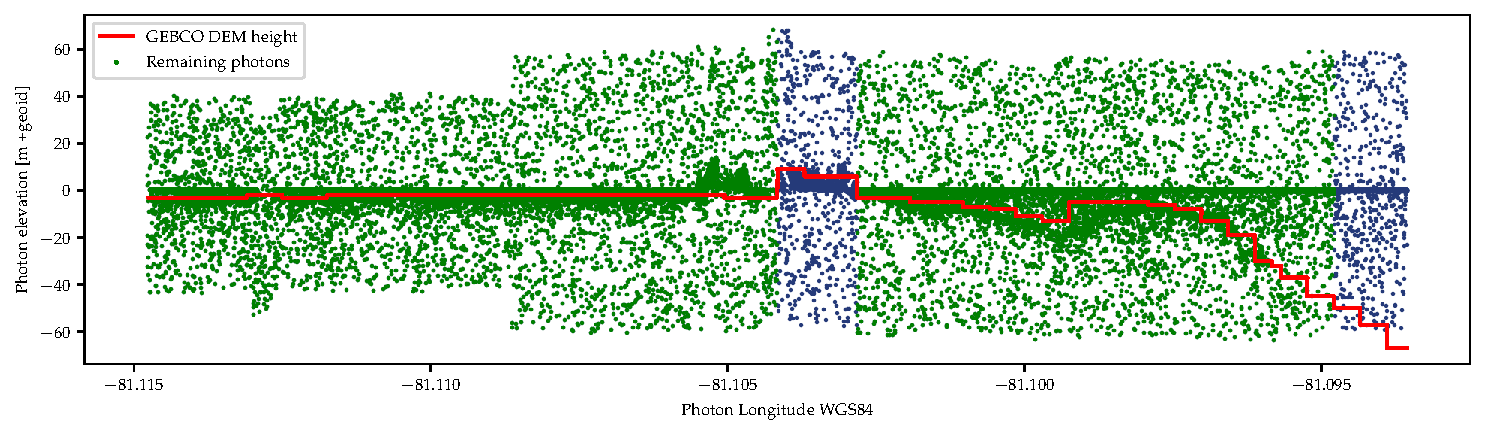
\includegraphics[width=\textwidth]{figures/methodology_gebco_filtering.pdf}
        \caption{The GEBCO data for the example transect, and the photons that are removed due to the GEBCO depth}
        \label{fig:gebco_filtering}
    \end{figure}

    \item The local sea-surface elevation $h_{sea}$ is calculated by taking the median elevation of the  high-confidence sea surface photons in the transect. The water depth for each photon is then calculated. The standard deviation of the elevation high-confidence photons $\sigma_{h_{sea}}$ is also calculated. This is used as a proxy to estimate the magnitude of the wave height at the time of the observation.
    \item Any photons with a water depth greater than 40 meters or a geoidal height less than -40m are removed, based on the same assumption that they are too deep to be bathymetric photons. 
    \item To remove the sea surface signal and any noise points above it, any photons that are higher than $h_{sea} - \max{(2.5\sigma_{h_{sea}},1~m)}$ are removed. This removes the sea surface signal and any high noise photons.
    
    The results of steps 2-4 are shown in figure \ref{fig:vert_filtering}
    
    \item As an additional check, any photons with a geoid height greater than 10~m are removed. This is justifiable because it does make make physical sense to find bathymetric photons that high above the geoid surface. This additional step is required because it was found that in Oahu there are some photons classified as high-confidence ocean signal with an elevation in the range 50-100~m. This is likely due to misclassification of cloud photons as ocean surface signal.
    
    
    \begin{figure}[htb]
        \centering
        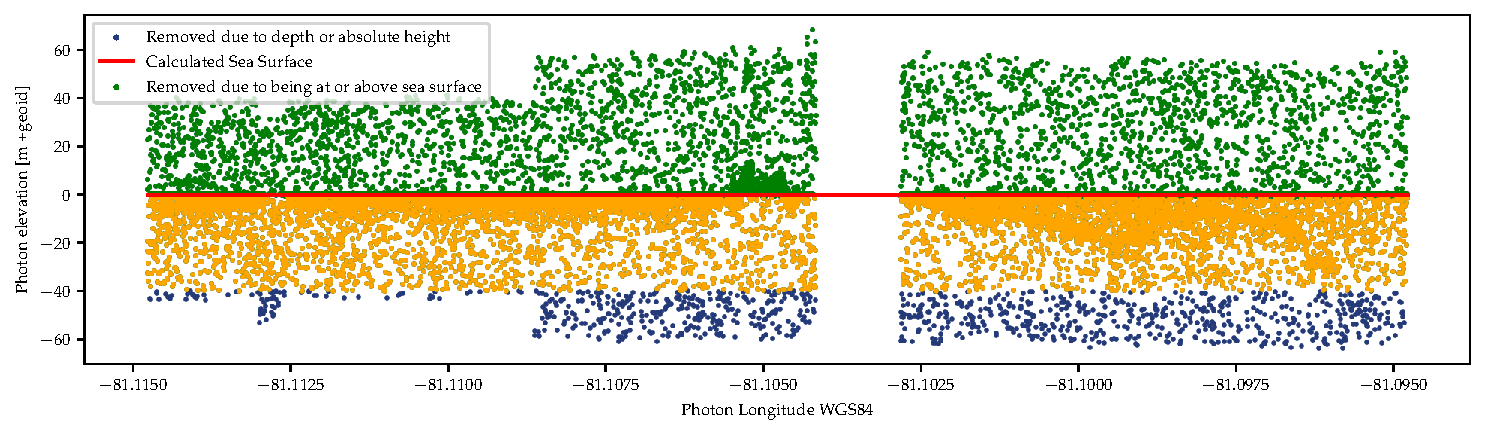
\includegraphics[width=\textwidth]{figures/methodology_sealvl_filtering.pdf}
        \caption{Vertical point filtering based on the local sea surface elevation}
        \label{fig:vert_filtering}
    \end{figure}
\end{enumerate}

After these filtering steps, the resulting subsurface photons for this example transect are shown in figure \ref{fig:remaing_photons}. The bathymetric signal can be seen clearly throughout the entire transect.

\begin{figure}[htb]
    \centering
    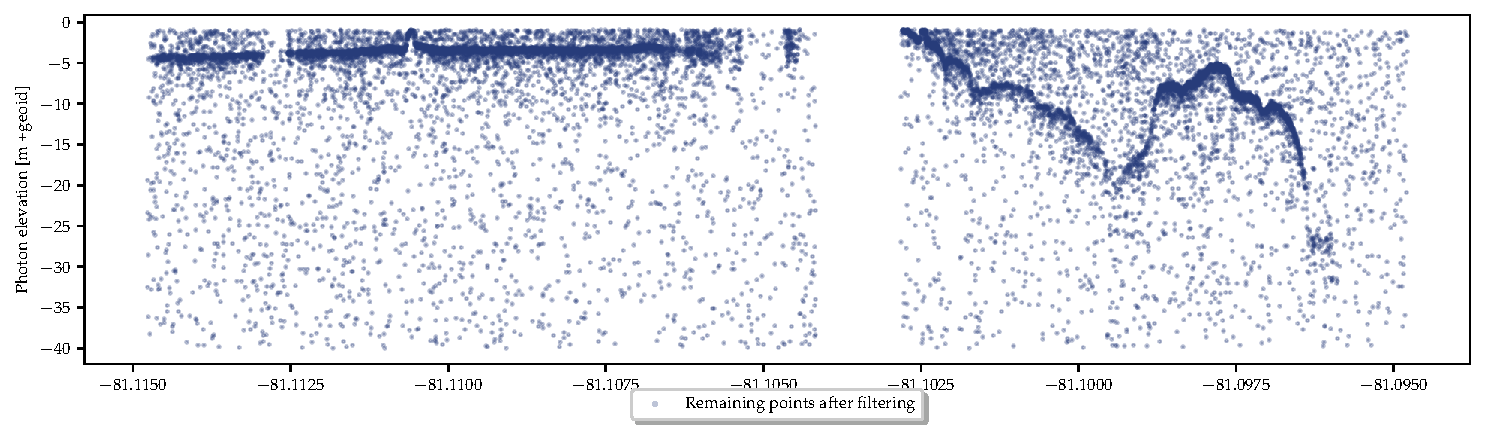
\includegraphics[width=\textwidth]{figures/methodology_reminaing_after_filtering.pdf}
    \caption{Subsurface photons found resulting after the filtering process}
    \label{fig:remaing_photons}
\end{figure}

An overview of the entire filtering chain is shown in Figure \ref{fig:filtering-flowchart} 

\begin{figure}[htb]
    \centering
    \includegraphics[]{figures/drawio/filtering_flowchart.pdf}
    \caption{Subsurface filtering overview}
    \label{fig:filtering-flowchart}
\end{figure}

Finally, before the signal-finding is applied, the Parrish method of refraction correction, including the correction factor for curvature of the earth, is applied to all subsurface photons. Figure \ref{fig:refraction-photons} shows the effect of the refraction correction step on the subsurface photons.

\begin{figure}[htb]
    \centering
    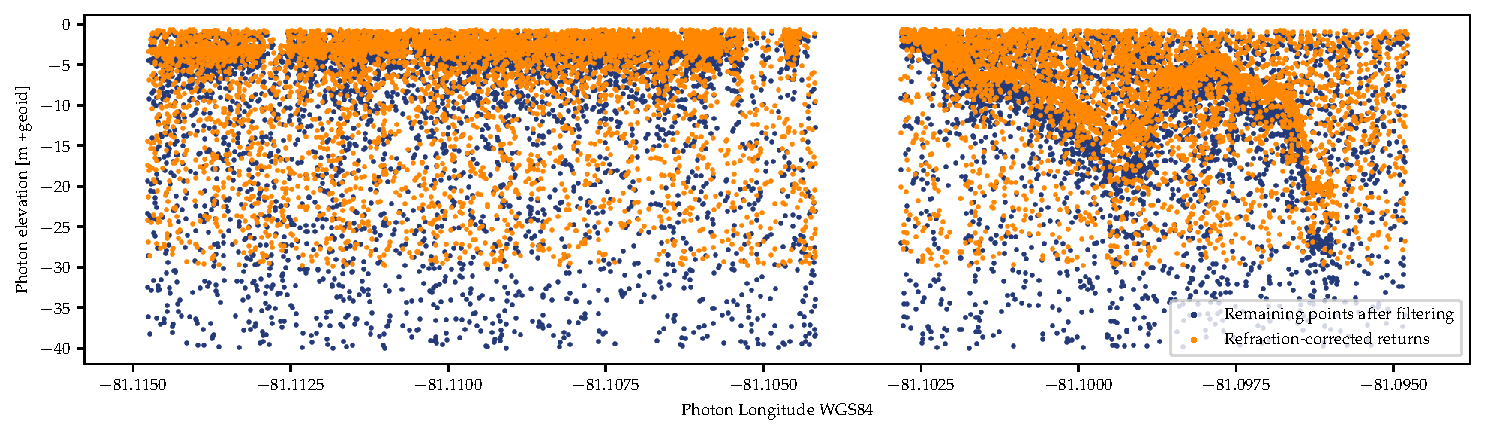
\includegraphics[width=\textwidth]{figures/methodology_refraction.pdf}
    \caption{The refraction correction applied to the remaining photons}
    \label{fig:refraction-photons}
\end{figure}

\subsection{Bathymetric signal extraction}\label{subsec:kdesignalfinding}

The filtering steps reduce the dataset to only photons that have been geolocated to the subsurface zone. However, there might not be any usable photon data in that zone. To determine if there is bathymetric signal present, further processing is required. Some proposed methods for separating bathymetric signal photons from noise are explained in section~\ref{subsec:signal-finding}. These approaches are all based on the same principle, namely that an increased density of photon returns in an area means that it is more likely to be bathtymetry signal. For this project, a method is proposed based on a gaussian Kernel Density Estimation (KDE) function, a non-parametric estimator of the local probability density. 

The KDE function is highly influenced by the \emph{bandwidth} parameter. For this implementation, the Scott method \parencite{Scott2015} is used to estimate the KDE bandwidth: $$ n^{\frac{-1}{d+4}} $$ where $n$ is the number of data points and $d$ is the number of dimensions of the data. 

A function is created that calculates the maximum kernel density, and the Z location at which it occurs. $$ f(\hat{z}_{window}) \rightarrow kde_{max},z_{kde_{max}} $$ This function is then applied across a rolling window of the transect. The rolling window is applied across the time dimension to 100 adjacent points. Figure \ref{fig:kdefunc} shows the KDE function as applied to a single example window, and the resulting kernel density plot of that window.

\begin{figure}[htbp]
    \centering
    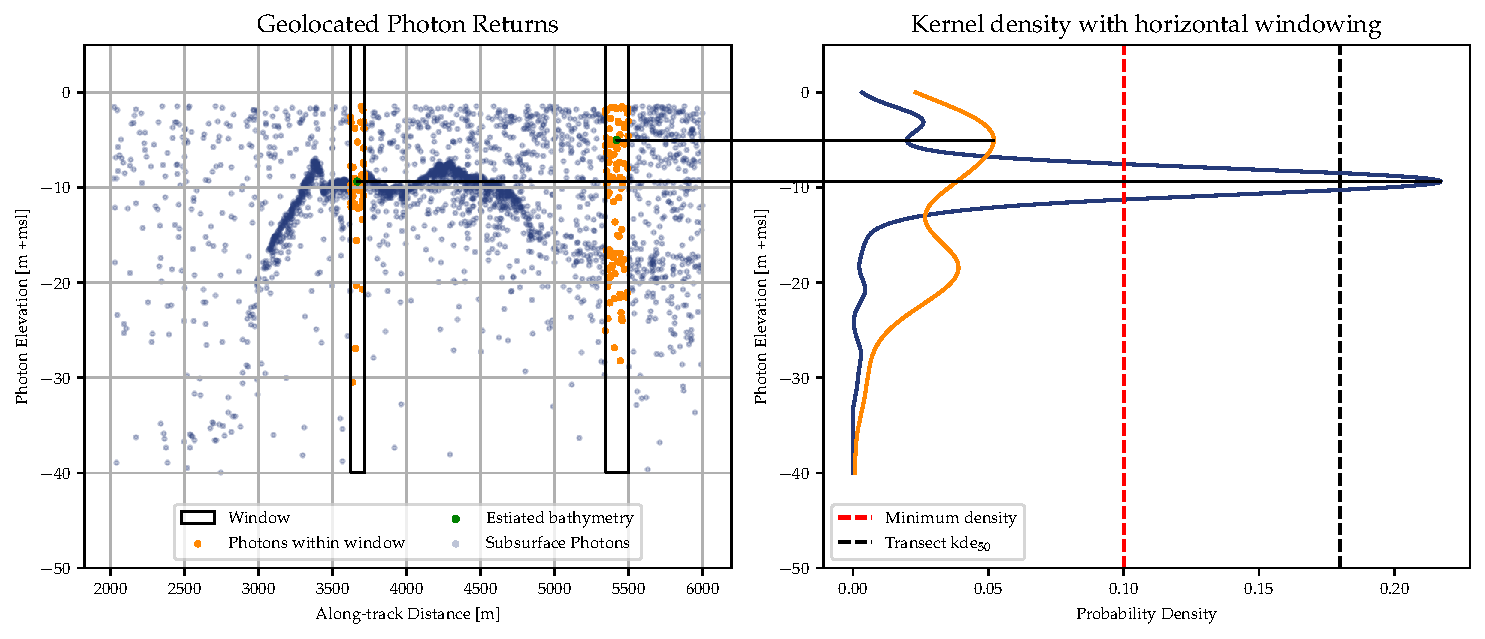
\includegraphics[width=\textwidth]{figures/2d_kde_plot.pdf}
    \caption{KDE function as applied to single window}
    \label{fig:kdefunc}
\end{figure}

This kernel density function gives an indication of the strength and location of the density peak for every photon in the transect. To reject locations where the signal is weak, a threshold needs to be established for a distinguish between signal and noise. Because there can be significant variation in the density value between different transects, this is set adaptively based on either the median kde value $kde_{50}$, or $kde_{min}$, whichever is greater. The absolute minimum threshold of $kde_{min}$ is required because some transects contain no useful bathymetric signal. Setting an absolute minimum ensures these transects are more likely to be rejected as noise. 

Any photons with a KDE value less than the threshold are assigned an NaN value and are dropped from the analysis and the remaining photons are saved for further use.

To summarize, the input parameters to the signal finding process are:

\begin{enumerate}
    \item The size of the window in number of adjacent points
    \item the minimum density value for the kernel density required for point to be considered signal
\end{enumerate}

Based on empirical analysis of the test sites, a window of 100 adjacent photons and a minimum density of 0.1 were found to provide good results when compared to validation data.

\subsection{Interpolation to a 2D grid}\label{subec:gridding}

After the bathymetric signal points are identified using the approach described in section \ref{subsec:kdesignalfinding}, the resulting bathymetry points are densely spaced along satellite tracklines, but are absent between them. A number of interpolation techniques have been applied to create bathymetry grids from point data. Commonly, inverse-distance weighting (IDW), tension splines, or loess interpolators have been used \parencite{gebcocookbook,Ferreira2017}. These approaches are relatively straightforward and easy to implement. However, the disadvantage of these simple approaches is that there is not a clear methodology of establishing the uncertainty of the resulting interpolation. Intuitively, areas with a higher point density will lead to an interpolation with a lower uncertainty that areas with very sparse points. Kriging is a geostatistical technique that allows interpolating points into a grid, while also giving an indication of the uncertainty in the neighborhood. By knowing both our estimated sea floor depth and the uncertainty in the estimate, we can use a Bayesian approach to update our initial guess of the seafloor location.


\subsubsection{Subsampling of bathymetric points using Poisson disk sampling} \label{subsec:poissonsubsampling}
The bathymetric points are extremely densely spaced in some areas and transects. This can present an issue to kriging, which is computationally expensive and points too close together can make the algorithm even slower. To reduce the number of points fed into the algorithm, a subsample of the points is taken using the Poisson disk sampling technique. Poisson disk sampling is a strategy that generates random samples of a distribution that are a minimum distance apart. When applied to a point cloud, in this case the point cloud of all the bathymetric points, the sampling function will only return points that are a minimum distance apart in 3d space. This ensures that the sampling is as representative as possible of the underlying surface.

The implementation used is from the PDAL software library \parencite{howard_butler_2022_6369164}, which provides an iterative Poisson disk sampling function based on \citeauthor{McCool1992} (\citeyear{McCool1992}). The disk sampling is applied iteratively with a decreasing radius until the desired number of points is reached. In this case, it was found that the maximum number of points that can be practically be used in the kriging step is approximately 2000 points. Therefore, this was the number of points used to allow the maximum possible point density while using a consumer-grade laptop to run the algorithm. 

\subsubsection{Kriging interpolation}
The subsample of points obtained from the poisson disk sampling is then interpolated into a grid format using a universal kriging approach. This geostatistical technique results in a grid of the estimated depth as well as the estimated uncertainty. 

The universal kriging interpolator used is a 2D interpolator, and both the estimated surface and its associated uncertainty are generated for the entire site. A single slice of the output, taken along an ICESat-2 transect, is shown in Figure \ref{fig:kriging-interpolator}. Note that the uncertainty estimate for the interpolated GEBCO surface is constant, and the uncertainty estimate for the kriging interpolator increases with increased distance from the measurement points. 

A spherical variogram with a range of $10 km$, a nugget variance of $0.7 m^2$, and a sill variance of $25 m^2$ was found to produce good results in most sites. The python package Pykrige \parencite{benjamin_murphy_2021_5380342} was used to implement the universal kriging approach. 

\begin{figure}[h]
    \centering
    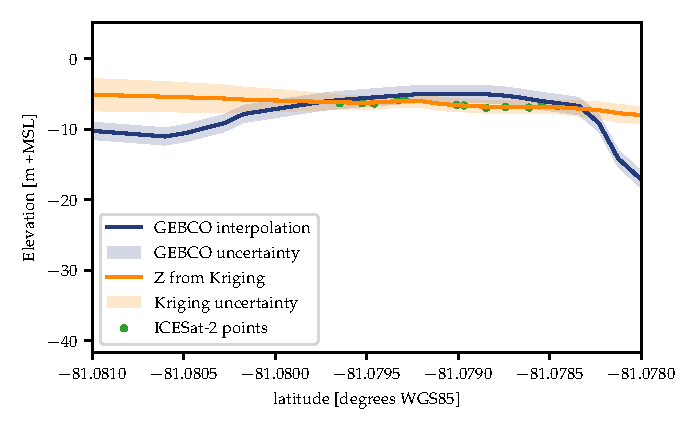
\includegraphics[]{figures/methodology-kriging-output.pdf}
    \caption{Example of the subsampled points, and the results of a kriging interpolation. In blue, the result of GEBCO is shown for comparison.}
    \label{fig:kriging-interpolator}
\end{figure}


\subsection{Bayesian data assimilation using Kalman update equation}\label{subsec:Kalman-update}

The Kalman Filter is a mathematical technique to predict the state of systems based on uncertain measurements. It consists of a loop of two steps, an \emph{time update} step which updates the position based on a measurement and a known measurement uncertainty, and a \emph{measurement update} step which predicts the state based on the dynamic equations of the system. The Kalman filter equations are used to estimate the state of a linear process for a state $x_k$ and a vector of measurements of the state $z_k$ \parencite{Welch2021a}.  It is assumed that the state of a system evolves according to the difference equation

\begin{equation}
 x_k = Ax_{k-1} + Bu_{k-1} + w_{k-1}   
\end{equation}

Where $A$ is a matrix that relates the state at time step $k$ to the state at the previous time step and $w_k$ represents normally distributed process noise with a variance $Q$.  

Measurements of the state are assumed to have the form

\begin{equation}
    z_k = Hx_k + v_k
\end{equation}

Where $H$ is a matrix that relates the state to the measurement, and  $v_k$ is measurement noise which is assumed to be normally distributed with a variance $R$.

At each time step $k$, the estimates of the state can be updated according to the following two steps:

Time Update:
\begin{equation}\label{eq:timeup1}
    \hat{x}_{\bar{k}} = A\hat{x}_{k-1} + B\hat{u}_{k-1}
\end{equation}

\begin{equation}\label{eq:timeup2}
    P_{\bar{k}} = A P_{k-1} A^T + Q
\end{equation}

Measurement Update:
\begin{equation}\label{eq:kalmangain}
    K = P_{\bar{k}} H^T(H P_{\bar{k}} H^T + R) ^{-1}
\end{equation}

\begin{equation}\label{eq:new_state_measurement}
    \hat{x}_k = \hat{x}_{\bar{k}} + K(\hat{z}_k - H \hat{x}_{\bar{k}})
\end{equation}

\begin{equation}\label{eq:new_uncertainty}
    P_k = (I - KH)P_{\bar{k}}
\end{equation}

Where:
\begin{itemize}
    \item $\hat{x}_k$ is the current state of the system
    \item $\bar{k}$ is the measurement matrix
    \item $P_k$ is the error covariance matrix
    \item $K$ is the Kalman gain
\end{itemize}

To apply this to this bathymetry estimation problem, some simplifying assumptions are made. The nearshore zone is a highly dynamic system. However, for the purposes of this project it is assumed that the temporal variations over the time scale being studied are within the margin of error of the measurements, so the bathymetry of the nearshore zone is assumed to be a static system and the time update equations \ref{eq:timeup1} and \ref{eq:timeup2}. 

Equation \ref{eq:kalmangain} is the Kalman gain, an estimation of the strength of the estimation. For this case, it is assumed that the matrix $H$ is the identity matrix. Equations \ref{eq:kalmangain}, \ref{eq:new_state_measurement}, and \ref{eq:new_uncertainty} can be simplified to 

\pdfcomment{number these?}
$$ K =  \frac{P_k}{P_k + R} $$

$$ \hat{x}_k =  \hat{x}_{\bar{k}} + K(\hat{z}_k -  \hat{x}_{\bar{k}}) $$


$$ P_k = (1 - K) P_{\bar{k}} $$


It is also assumed all measurements are measurements of the same underlying physical depth, and that differences between measurements are due to normally distributed measurement error, with magnitude of the error varying depending on the method. To combine multiple measurements, the \emph{measurement update} step is applied recursively for each available measurement to produce and updated estimate of the bathymetry grid. This is a Bayesian update, in that it considers the uncertainty of each measurement when combining them. 

In this application, the starting point of estimate is based on a bilinear resampling of the GEBCO dataset, with an assumed variance of $1.5~\text{m}^2$. The value was found empirically to give good results in most test sites. Then, the simplified Kalman equations above are applied. At each raster grid cell the kriging uncertainty is used As $R$, and the kriged estimate of the seafloor is used as $\hat{z}_k$. The result is a new estimate of the bathymetry that includes both the kriged lidar surface and a priori depth of GEBCO. Figure \ref{fig:Kalman-figure} shows both the output of the kriging process, including the uncertainty bars for each. The plot on the left side shows the estimated probability density functions of the bathymetry surface along the black vertical line. The green PDF curve, labeled \emph{a posteriori estimate} shows the resulting of Kalman update along that slice.

\begin{figure}[htb]
    \centering
    \includegraphics[width=\textwidth]{figures/methodology-Kalman-updating.pdf}
    \caption{Using a section of the same transect in Figure \ref{fig:kriging-interpolator}, the processing of the Kalman measurement update is shown}
    \label{fig:Kalman-figure}
\end{figure}

\subsection{Per-track Secchi disk depth estimation}
To evaluate the relationship between the Secchi disk depth at the location and the time of the transect, and the quality of the bathymetry estimate, the Secchi depth value from the GlobColour dataset \parencite{Garnesson2019} is found at points distributed along each ICESat-2 transect. 

The GlobColour Daily Secchi Depth dataset is provided at a 4km horizontal resolution, and a 1 day temporal resolution. To calculate the Secchi depth in water areas at the time of the satellite pass, the ATL03 tracklines are divided into points every $4~\text{km}$ starting at the end of the transect. For each of these points, the closest ocean color data in time and space is calculated using Xarray. 

One issue is that this approach generates some points over land. The GlobColour data does include a land mask, but because of the $4~\text{km}$ horizontal resolution of the ocean color product, the land mask is not reliable along coasts. However, the GEBCO dataset has a much higher horizontal resolution than the GlobColour data ($450~\text{m}$). Therefore, in this case the GEBCO data can be used as a land mask. For each Secchi disk depth point, the corresponding GEBCO elevation is found, and if it is greater than 0 the point is assumed to be on land and is rejected. 

This provides a dataset of the water clarity (as estimated by Secchi disk depth) data at the location and day of the satellite pass. Ocean color statistics can then be calculated for each unique trackline, or for a site as a whole.


\subsection{Error evaluation}

To compare the results to the validation data, several different error metrics are considered. Both the error between the validation data and the lidar data is checked to evaluate the performance of ICESat-2 measurements, and the signal finding algorithm, and the total decrease in error between GEBCO and the version of GEBCO that includes the interpolated ICESat-2 data. 

The error metrics that are evaluated for both types of error are the root mean square error (RMSE) and the mean absolute error (MAE). The RMSE is calculated by taking the mean of the squared difference between the true value and the estimated value, and then taking the square root of this mean.

$$  \text{RMSE} = \sqrt{\frac{1}{n}\Sigma_{i=1}^{n}{\Big(\frac{x_i - y_i}{\sigma_i}\Big)^2}}  $$

By squaring the error first, larger magnitude errors are given relatively more weight in the metric. Mean absolute error also gives an idea of the average deviation, but gives equal weight to all errors.

$$ \text{MAE} = \sum_{i=1}^{D}|x_i-y_i| $$

To evaluate these errors between the Kalman-updated bathymetry grid and the validation data reprojection and resampling is required. The validation data has a horizontal resolution on the order of 1m, while GEBCO has a horizontal resolution on the order of 450m. Before taking the error, the data being compared is first reprojected into the native coordinate system and resolution of the validation data using GDAL \parencite{rouault_even_2022_6352176}. Then, the RMSE and MAE can be calculated between each cell of the raster grid.

The coefficient of determination $R^2$ can evaluated between the ICESat-2 bathymetry estimates and the true elevation at the corresponding point. It gives an indication of how well a ICESat-2 bathymetric photon value without a known ground-truth elevation would be predicted by the approach. This metric is given by the formula:

\begin{equation}
    R^2 = 1 - \frac{\sum_{i=1}^{n} (x_i - y_i)^2}{\sum_{i=1}^{n} (x_i - \bar{y})^2}
\end{equation}


\section{Possible limitations}

This section introduces some possible soures inherent limitations or error in the method, and how how they are mitigated if at all.

\subsection{Limitations in Photon Geolocation Accuracy}

The pointing determination algorithm used by the satellite has a high vertical accuracy, but there is an inherent limitation on the horizontal accuracy. The current best estimate of the vertical accuracy is 0.17cm, and the estimate of the x and y position uncertainty is 5m \parencite{Neumann2019c}.

This uncertainty, and the horizontal refraction, are more likely second order effects. Because the kriging is used to create a product of 50m resolution, any uncertainty introduced by this will be masked by the interpolation to a 50m grid.

\subsection{Errors in refraction correction}

The refraction correction method used accounts for the additional horizontal error that is introduced by off-pointing. However, there are several other second-order effects that are not considered by the methodology. One of these is the estimation of the refractive index; the temperature and salinity affect the speed at which the water transmits light. By assuming a default value, it could introduce some error in sites that deviate significantly from the assumed default. This effect was deemed likely a second order effect and was not considered here. However, this could be corrected by either looking up the appropriate values for each site beforehand, or by connecting the algorithm to an API that can provide a temperature and salinity value for any site and time.

Another potential source of error is the slope of the water surface. Since there is a slope to the water surface, this affects the bounce angle of the photon. This can be corrected for and some papers that investigate ICESat-2 bathymetry have attempted to correct for it. For this project the magnitude of error due to slope was considered small enough to be within the margin of error of the method.

\subsection{Misclassified photons in ATL03 data}

Correct filtering of sea surface returns is very important to the accuracy of the bathymetry signal finding, because the sea surface signal is often several orders of magnitude more dense than the bathymetric signal, and the location of the sea surface is also used to calculate the depth of a photon for refraction correction. The default photon classification provided in the ATL03 data is used to identify the sea surface within the filtering algorithm. Errors in the default ocean signal classification can result in sea surface signal being inadvertently included in the subsurface data and biasing the KDE results.

The default classification is often reliable, but when there is a large area where the bathymetric surface is shallow and nearly parallel to the sea surface, there can be misclassifications. An example of this is shown in figure \ref{fig:ageeba_bad_classes}. In this example, actual sea surface is not classified as a high confidence ocean surface return, and some areas that appear to be bathymetric signal are classified as ocean surface. This causes the bathymetric signal to be thrown out because it is incorrectly considered to be the sea surface.

This could potentially be mitigated by a different filtering strategy that calculates the local sea surface based on the local geoid. This could be very feasible in microtidal areas where the tidal signal has a smaller impacts.

% \pdfcomment{temp figure, replace with matplotlib figure with axis labels. Maybe also include a plan view map with scale bar to understand the geographic context}
\begin{figure}[htbp]
    \centering
    \includegraphics[width=\textwidth]{figures/ageeba_beach_example.png}
    \caption[Misclassification errors example]{Classification of photons from 2021-07-19, Beam gt3r, reference ground track 396. This transect is located off the coast of Egypt. The two parallel straight lines from 200 to 800 are the sea surface and the bathymetric signal. The NASA photon classification algorithm misclassifies the bathymetric points as ocean surface returns}
    \label{fig:ageeba_bad_classes}
\end{figure}


\subsection{Limited spatial coverage in some islands}

In support of the vegetation mission of ICESat-2, the instrument is sometimes pointed as much as several degrees to the side of the reference ground tracks when the satellite passes over land. This increases the spatial density of points at the expense of the temporal resolution. For bathymetric purposes the increased spatial resolution gives a more even coverage of nearshore zone bathymetry. 

However, the land mask that is used by NASA to determine the off-pointing strategy has a limited resolution, and therefore some island nations do not benefit from the increased spatial density. This was noted when trying to collect data from Fiji and the Maldives. Due to apparently being located within the off-pointing zones, both of the aforementioned islands only have tracks which are 3km apart. They can still potentially collect bathymetry data if conditions are otherwise good, but the further reduction in spatial coverage limits the accuracy of the kriging method. This is unfortunate because many of the states that are at the highest need of detailed bathymetry for numerical studies are big ocean island nations. The tradeoff for this scenario is that the temporal resolution is significantly better, so the spaceborne lidar could be useful for studying the changes over time. 

\subsection{Inherent uncertainty of KDE Method}
There are a number of input parameters to the filtering and the density-based bathymetry finding methods. These parameters can be optimized for each site to reduce the RMS error as much as possible if there is some validation data available. However since the end goal of the project is to be able to improve estimates without using any in situ data, ideally there would be no need for optimization based on the site.

Currently the globally-set parameters are sufficient to extract bathymetry without any tuning for all of the case studies that are investigated. However, the inability to tune in advance is a limitation. 

One possible future step would be to gather even more validation sites, and explore which other variables might influence the best parameter setting. It is possible that there are certain site variables which predict the optimal parameter options. Even so, upscaling of validation sites would allow better insight into which variables predict the presence of valid data.  

\subsection{ATL03 data quality issues}\label{sec:discussion-photon-issues}

There are a number of known issues with the ICESat-2 data. They are either due to atmospheric and environmental conditions, or due to limitations of the instrument. Many of them can be detected in advance, and then the effected granule data can be thrown out or the issue otherwise corrected for. However, there might be some edge cases related to these issues that cause either false bathymetric signal points, or cause the algorithm to miss valid bathymetric data. These data issues could present an issue for the scaling up the signal finding without any manual intervention. Currently the process is run without any intervention, but the sites are small enough to manually check several of the transects.

The following known data issues could effect the results of the KDE signal finding algorithm:

\subsubsection{Clouds}

The presence of some clouds along a single granule can cause the loss of data that might otherwise be valid

Clouds reflect sunlight which causes a higher background photon rate, and this can create issues with the telemetry bands and cause the telemetry bands to not include the surface. Even if the actual earth surface is included in the telemetry band, the clouds can affect the travel times and create inaccurate readings \parencite{atl03knownissues}.

During processing from L0 to L1, if the elevation from NASA reference DEM is not within the telemetry bands, no photons will be classified as signal. Therefore, if the entire granule is affected by this issue, there will be no sea surface found and therefore the entire granule will be filtered out. This can cause a significant loss of data but it is an issue inherent to nearly any remote-sensing based approach. One possible way to mitigate this would be to combine the ICESat-2 bathymetry data with synthetic aperture radar (SAR) remote sensing data. SAR remote sensing data can penetrate clouds because it uses radiometry outside of the visible spectrum. Although the spectrum used in SAR sensing cannot directly penetrate even clear water, the data can be used to estimate wave conditions, and the bathymetry can be estimated based on the transformation of the wave (called \emph{wave kinematic satellite-derived bathymetry}). The bathymetry estimates from SAR-derived wave kinematic SDB could be incorporated into the Kalman filtering step. 

In situations where the photons are able to pass through clouds, the changes to travel time through the clouds can affect the accuracy. This could potentially be something that is hard to detect and affect the accuracy of the bathymetric points if any are found.
 

\subsubsection{Multiple Telemetry Bands}

If the signal detection on board the satellite cannot determine where the primary surface is located, it will open another telemetry band to try to collect more signal. This can create other areas of photons that are significantly above or below the surface.

